\problemname{Safest Taxi}

Consider a town whose road network forms an $N * M$ grid, where adjacent intersections are connected by roads. All roads are bi-directional. Each direction has an associated number - the time needed to travel from one end-point to another.

Each direction of each road consists of one or more lanes. A lane can serve one of the following functions: left-turn, straight, right-turn, or any combination of them. However, a left-turn lane cannot be placed to the right of a straight or right-turn lane, and a straight lane cannot be placed to the right of a right-turn lane. There are no U-turn lanes.

\begin{center}
	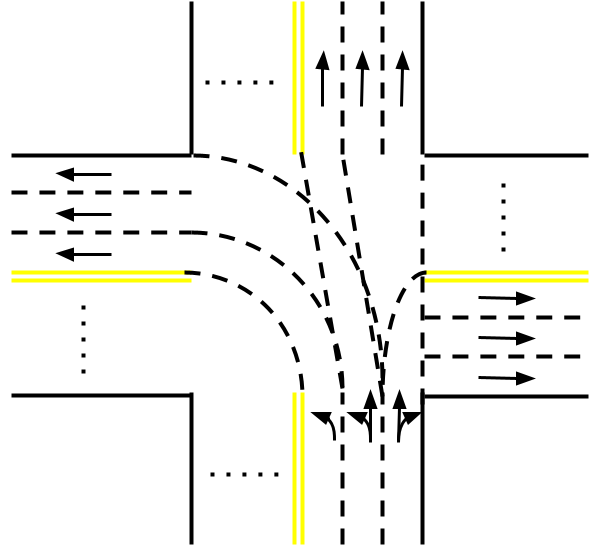
\includegraphics[width=0.4\textwidth]{illustration.png}
\end{center}

The rules for crossing intersections are illustrated in the above figure (suppose a car enters the intersection from the south). To make a left turn, it must be in one of the $L$ left-turn lanes; let's number them $1$ through $L$ from left to right. The traffic rule says Lane $i$ must turn into the $i$-th lane (counting from the left) of the target road, except that Lane $L$ may turn into the $L$-th lane or any other lanes to its right. 

Similarly, to go straight through an intersection, the car must be in one of the $S$ straight lanes; let's number them $1$ through $S$ from left to right. Lane $i$ must go into the $i$-th lane (counting from the left) of the target road, except that Lane $S$ may go into the $S$-th lane or any other lanes to its right.

To make a right turn, the car must be in one of the $R$ right-turn lanes. For the convenience of discussion, we consider these lanes and those of the target road {\it from right to left}. Let's number the right-turn lanes $1$ through $R$ from right to left. Lane $i$ must turn into the $i$-th lane (counting from the right) of the target road, except that Lane $R$ may turn into the $R$-th lane or any other lanes to its left.

It is guaranteed that if at least one left-turn / straight / right-turn lane is present, the target road must exist and have enough lanes to accommodate the left turn / straight / right turn, respectively. The time spent on crossing intersections is negligible.

In addition, a driver may change lanes in the middle of a road. Note that in the above rules for intersections, it doesn't count as a lane change to drive into any of the legal lanes of the target road. The time spent on lane changes is negligible.

A trip starts and ends at the rightmost lane of the midpoint of roads. The time needed to travel midpoint-to-endpoint is half of endpoint-to-endpoint.

You are running a taxi company called ``Safest Taxi'' in this town, with the slogan ``your safety is in your hands''. You let your customers choose the numbers $X$ and $Y$ for their trip, and the driver will make at most $X$ left turns and $Y$ lane changes to accomplish the trip.

What is the shortest time to fulfill each trip given the rules?

\section*{Input}

The first line consists of three integers $N$ ($2 \leq N \leq 15$), $M$ ($2 \leq M \leq 15$) and $K$ ($1 \leq K \leq 3$), separated by a single space. The town's road network has $N$ intersections north-south and $M$ intersections west-east. Each road has $K$ lanes.

The second line consists of a single integer $D$. The town's road network has $D$ road segments. Every adjacent pair of intersections must appear in the list exactly once.

Each of the next $D$ lines describes a road segment with the following format:

$$R_0\;C_0\;R_1\;C_1\;T\;L_0\;L_1 ... L_{K-1}$$

This describes a road segment going from the intersection at row $R_0$ column $C_0$ to the intersection at row $R_1$ column $C_1$ ($0 \leq R_0,R_1<N$, $0 \leq C_0,C_1<M$). Rows are numbered $0$ through $N-1$ from north to south, and columns are numbered $0$ through $M-1$ from west to east. The segment must connect two adjacent intersections, i.e., $\mid R_0 - R_1 \mid + \mid C_0 - C_1\mid  = 1$. The time to travel through the entire segment is $T$ ($2 \leq T \leq 100$, $T$ must be an even number). The next $K$ strings describe the function of each of the $K$ lanes, from left to right, with the following semantics:\vspace{.5em}

  L   $\mid$ Left-turn only

  S   $\mid$ Straight only

  R   $\mid$ Right-turn only

  LR  $\mid$ Left-turn or right-turn

  LS  $\mid$ Left-turn or straight

  SR  $\mid$ Straight or right-turn

 LSR  $\mid$ Left-turn, straight or right-turn\\

The next line consists of a single integer $P$ ($1 \leq P \leq 50$), the number of trips to fulfill.

Each of the next $P$ lines describes a trip with the following format:

$$R_{S0}\;C_{S0}\;R_{S1}\;C_{S1}\;R_{D0}\;C_{D0}\;R_{D1}\;C_{D1}\;X\;Y$$

This indicates that the starting point is the midpoint of segment ($R_{S0}, C_{S0}$) $\to$ ($R_{S1}, C_{S1}$), and the destination is the midpoint of segment ($R_{D0}, C_{D0}$) $\to$ ($R_{D1}, C_{D1}$). Both segments must appear in the above list. Both the starting point and the destination are on the rightmost lane. The customer requests that at most $X$ ($0 \leq X \leq 4$) left turns and $Y$ ($0 \leq Y \leq 4$) lane changes are allowed for the trip.

\section*{Output}

Output $P$ lines. The $i$-th line contains a single integer which is the shortest time to fulfill each trip given the rules, or $-1$ if no feasible route exists.

\section*{Sample Explanation}

The first three lines of the sample output are illustrated in the figure below.

\begin{center}
	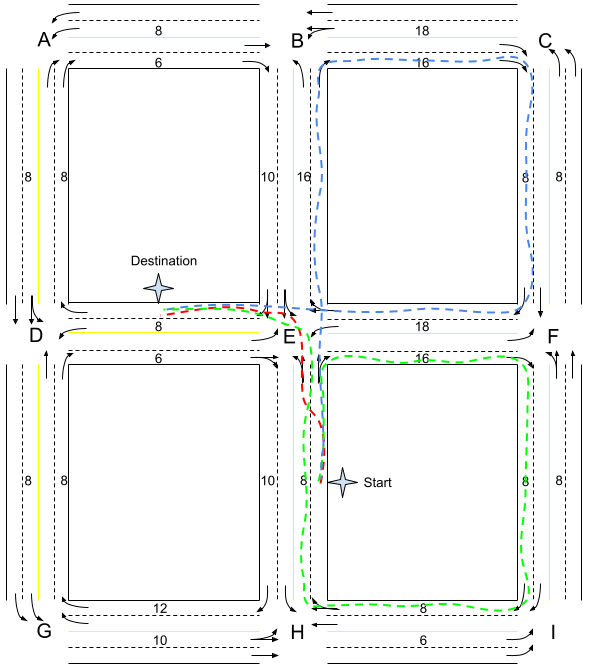
\includegraphics[width=0.9\textwidth]{figure.png}
\end{center}

\begin{itemize}
\item If $X = 1$ and $Y = 1$, the shortest path is shown in red: make a lane change before reaching E and make a left turn. The total time is $8/2+8/2=8$;
\item If $X = 1$ and $Y = 0$, the shortest path is shown in green: go through E-F-I-H-E and make a left turn. The total time is $8/2+16+8+8+8+8/2=48$;
\item If $X = 0$ and $Y = 0$, the shortest path is shown in blue: go through E-B-C-F-E. The total time is $8/2+16+16+8+18+8/2=66$.
\end{itemize}
